\subsubsection{Progress}
Over the past weeks, I have been working to optimize the floating point arithmetic unit I had initially made for the purpose of multiplying weights and biases in the neural network that we are building. Since I have since built a working addition module that works well except for certain edge cases such as inputs of infinity and NaN. Similarly I had built a multiplication unit based on research I had done. The multiplication unit is built to be more robust against these edge cases as I have built in filters to check the inputs before processing is done on them.\newline

The issue with the multiplication unit is that it uses the $*$ operator to perform the multiplication of the mantissa of each input. This is not necessarily good because uses these mathematical operations will cause the FPGA to perform them using a separate unit for maths rather than look up tables. We would like for the floating point modules to use look up tables because the maths unit can vary from FPGA to FPGA but the LUTs are share a great amount of similarity that would allow us to worry less with some of the more specific specifications of the FPGA we would like to use.\newline

While looking for solutions around this problem, I tried two different methods of pipelining both modules. My initial method was to create a pipeline module as shown in Figure \ref{fig:pipeline_module}. It can be seen that it is a standard pipeline module where the input and output are packed arrays with parameterised width and length. This feature was important because I intended to use it for both the addition and multiplication units and they have different register sizes. Upon further research, I found a better way to do pipelining that allowed for the register names to be more descriptive which allowed for easier debugging. Instead of using combinational blocks to perform logic, I instead used \texttt{always\_ff} (sequential blocks) to perform logic with the condition of \texttt{posedge clk}. \newline

Another solution I had for multiplication was to use a fixed iteration for loop to perform multiplication in the same way long multiplication is performed. This is shown in Figure \ref{fig:binary_multiplication}. It involves multiplying \texttt{input\_1} by \texttt{input\_2} 10 times (because the mantissa is 10 bits wide) after shifting \texttt{input\_2} left by one space on each iteration and adding all the results together. In the end we decided against this as a team and decided to continue to use the $*$ operator for multiplication. This makes debugging easier. 

\begin{figure}[H]
    \centering
    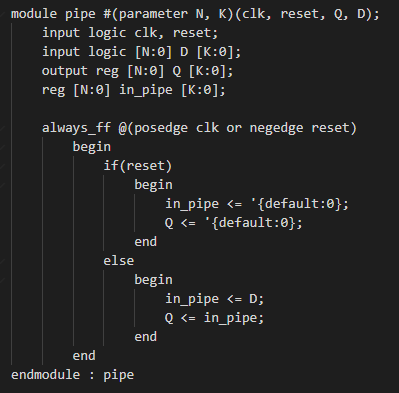
\includegraphics[scale=0.85]{resources/pipeline_module.PNG}
    \caption{Pipeline Module}
    \label{fig:pipeline_module}
\end{figure}

\begin{figure}[H]
    \centering
    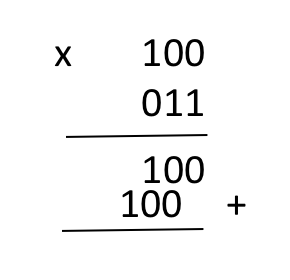
\includegraphics[scale=0.85]{resources/multiplication2.PNG}
    \caption{Binary Multiplication}
    \label{fig:binary_multiplication}
\end{figure}

\subsubsection{Difficulties Encountered}
Upon testing the multiplication unit I saw that the accuracy of the logic was not good enough to be used in the neural network. I had noticed that that was a marginal error with each result. In the cases where the result was within $0>|x|>1$, the error was a small percentage of the result ($<1\%$). On the other hand, when the result was large (>100) then the error would become a large percentage of the result (up to 20\% in some cases). As stated in the \textit{Progress Section} I attempted a different algorithm used to calculate the multiplication but it gave similar results. \newline

The multiplication unit has been pipelined and a test bench for it has been created. I am in the process of debugging the multiplication unit finding the right algorithm. Currently, I have been attempting to use the algorithm used in the IEEE 754 standard 32 bit multiplication module and scaling this down for 16 bit use. This still needs to be debugged and tested. 